% ============================================================================
%  cascade_forge — 1M-cell synthetic validation of cascadir direction inference
%  Build:  pdflatex report && pdflatex report
% ============================================================================
\documentclass[11pt,a4paper]{article}

\usepackage[margin=1in]{geometry}
\usepackage[T1]{fontenc}
\usepackage[utf8]{inputenc}
\usepackage{lmodern}
\usepackage{microtype}
\usepackage{amsmath}
\usepackage{booktabs}
\usepackage{graphicx}
\usepackage{xcolor}
\usepackage{caption}
\usepackage{tikz}
\usetikzlibrary{positioning,arrows.meta,calc}
\usepackage[colorlinks=true,linkcolor=blue!55!black,urlcolor=blue!55!black,
            citecolor=blue!55!black]{hyperref}
\graphicspath{{./}}

\definecolor{methodblue}{HTML}{0072B2}
\definecolor{ctrlorange}{HTML}{E69F00}

\title{\textbf{Forging ground truth: a one-million-cell synthetic validation
of single-snapshot cascade-direction inference}}
\author{Yam Arieli}
\date{July 9, 2026}

\begin{document}
\maketitle

\begin{abstract}
\noindent
\texttt{cascadir} infers the \emph{direction} of a signalling cascade from a single
single-cell snapshot, with no time course, by reading the asymmetric cross-presence of
discovered gene signatures (\texttt{cross\_asym}). On real data its direction calls can
only be checked against a handful of literature-audited pairs. Here we build
\texttt{cascade\_forge}, a small, pip-installable simulator that turns a
\emph{user-authored} cascade graph (edge strengths and pseudo-time delays) into a
single-cell snapshot with \emph{known} ground truth, and use it to benchmark
\texttt{cascadir} at scale: $10$ donors $\times\,20$ labels ($+$PBS) $\times\,5000$
cells per tube $=\,1{,}050{,}000$ cells. After correcting a benchmark-design confound we
introduced and caught (upstream labels were alphabetically ordered), \texttt{cross\_asym}
recovers direction at \textbf{100\%} ($90\%$ at the weakest perturbation), while the
symmetric control it is measured against sits at \textbf{$\sim$50\% (chance)} --- the same
contrast the method shows on real data, now on controlled ground truth. We also quantify
a weak-but-detectable effect-size floor ($\sim$0.15--0.20 in log space) and an honest
coupling over-call rate on isolated negative-control labels.
\end{abstract}

\section{Goal}
The method (\texttt{cross\_asym}) rests on a simple asymmetry: if $X$ lies upstream of
$Y$, cells given $X$ carry \emph{both} $X$'s own signature and the induced (autocrine)
$Y$ signature, whereas cells given $Y$ carry mainly their own. Comparing how much of each
signature appears in the other condition therefore points from upstream to downstream:
\[
  \mathrm{cross\_asym}(a,b) \;=\; s(a,S_b) - s(b,S_a),
\]
which is \emph{antisymmetric} ($\mathrm{cross\_asym}(b,a)=-\mathrm{cross\_asym}(a,b)$), so
its sign encodes direction. Its symmetric counterpart, \texttt{directional\_score}, cannot
encode direction and serves as a control that should sit at chance. The purpose of this
experiment is to test both against a cascade structure we author ourselves, so ``correct''
is known rather than inferred from literature.

\section{Methods}

\subsection{The simulator}
\texttt{cascade\_forge} takes a nested dict \texttt{\{source: \{downstream:
(strength, pseudo\_time\_delta)\}\}} and produces an \texttt{AnnData} snapshot that meets
the \texttt{cascadir} data contract (a condition column with one control label,
\texttt{PBS}; a donor column; a cell-type column). Generation proceeds in three stages:
\begin{enumerate}\itemsep2pt
  \item \textbf{Pseudo-time propagation.} For each applied label, seed only it (clamped
  on) and integrate first-order kinetics through the graph: each edge $X\!\to\!Y$ with
  $(w,\tau)$ ramps $Y$'s activation toward $w\cdot a_X$ with time constant $\tau$. Multi-hop
  cascades therefore emerge \emph{in order} and chain strengths multiply at steady state.
  \item \textbf{Planting.} A dominant cell-type marker signature ($\approx\!1.2$ over a
  $0.30$ baseline, log space) plus a deliberately \emph{weak} additive per-label program
  (\texttt{effect\_size}, $\ll$ the marker gap) scaled by each label's activation. The
  upstream label's cells thus carry both programs; the downstream label's carry only their
  own --- the asymmetry \texttt{cross\_asym} reads.
  \item \textbf{Output.} One snapshot \texttt{AnnData} per requested pseudo-time, raw
  Poisson counts (stored sparse), ground truth in \texttt{adata.uns}.
\end{enumerate}

\subsection{Authored cascade graph}
The graph (Figure~\ref{fig:system}) is designed to exercise every regime the method must
handle: a depth-3 chain, a shorter chain, a fan-out with mixed delays, a fan-in, a
feedback loop (excluded from signed scoring), and four \emph{isolated} negative-control
labels with no cascade. Configuration is summarised in Table~\ref{tab:config}.

\begin{figure}[h]
\centering
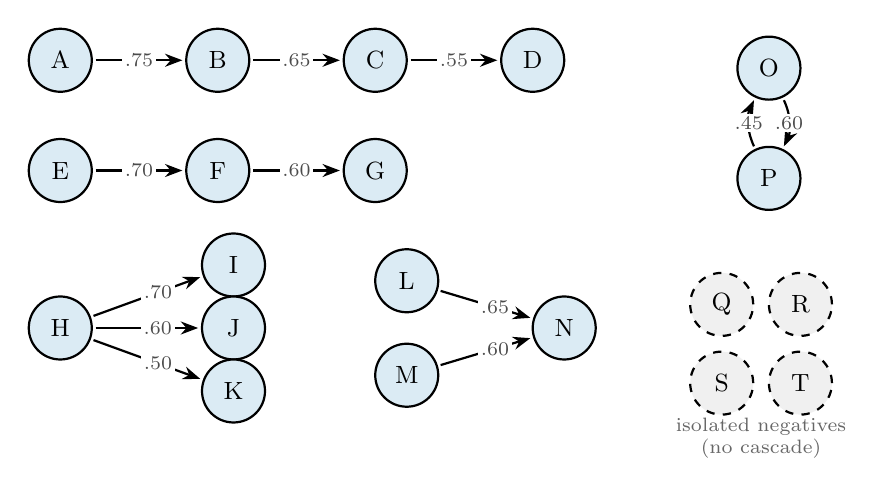
\begin{tikzpicture}[
  >={Stealth[length=2.2mm]},
  cnode/.style={circle,draw,thick,minimum size=8mm,fill=methodblue!14,font=\small},
  inode/.style={circle,draw,thick,dashed,minimum size=8mm,fill=black!6,font=\small},
  edg/.style={->,thick,shorten >=1pt,shorten <=1pt},
  elab/.style={font=\scriptsize,inner sep=1pt,fill=white,text=black!70}]

  % deep chain A->B->C->D
  \node[cnode] (A) at (0,5)   {A};
  \node[cnode] (B) at (2,5)   {B};
  \node[cnode] (C) at (4,5)   {C};
  \node[cnode] (D) at (6,5)   {D};
  \draw[edg] (A)--(B) node[elab,midway]{.75};
  \draw[edg] (B)--(C) node[elab,midway]{.65};
  \draw[edg] (C)--(D) node[elab,midway]{.55};

  % chain E->F->G
  \node[cnode] (E) at (0,3.6) {E};
  \node[cnode] (F) at (2,3.6) {F};
  \node[cnode] (G) at (4,3.6) {G};
  \draw[edg] (E)--(F) node[elab,midway]{.70};
  \draw[edg] (F)--(G) node[elab,midway]{.60};

  % fan-out H->{I,J,K}
  \node[cnode] (H) at (0,1.6) {H};
  \node[cnode] (I) at (2.2,2.4) {I};
  \node[cnode] (J) at (2.2,1.6) {J};
  \node[cnode] (K) at (2.2,0.8) {K};
  \draw[edg] (H)--(I) node[elab,pos=0.6]{.70};
  \draw[edg] (H)--(J) node[elab,pos=0.6]{.60};
  \draw[edg] (H)--(K) node[elab,pos=0.6]{.50};

  % fan-in {L,M}->N
  \node[cnode] (L) at (4.4,2.2) {L};
  \node[cnode] (M) at (4.4,1.0) {M};
  \node[cnode] (N) at (6.4,1.6) {N};
  \draw[edg] (L)--(N) node[elab,pos=0.6]{.65};
  \draw[edg] (M)--(N) node[elab,pos=0.6]{.60};

  % feedback O<->P
  \node[cnode] (O) at (9,4.9) {O};
  \node[cnode] (P) at (9,3.5) {P};
  \draw[edg] (O) to[bend left=25]  node[elab,midway]{.60} (P);
  \draw[edg] (P) to[bend left=25]  node[elab,midway]{.45} (O);

  % isolated negatives
  \node[inode] (Q) at (8.4,1.9) {Q};
  \node[inode] (R) at (9.4,1.9) {R};
  \node[inode] (S) at (8.4,0.9) {S};
  \node[inode] (T) at (9.4,0.9) {T};
  \node[font=\scriptsize,text=black!60,align=center] at (8.9,0.2)
        {isolated negatives\\(no cascade)};
\end{tikzpicture}
\caption{\textbf{The authored cascade system.} Nodes are labels; directed edges are
cascade relations annotated with strength. Solid blue: labels in a cascade (a depth-3
chain $A\!\to\!B\!\to\!C\!\to\!D$, a chain $E\!\to\!F\!\to\!G$, a fan-out
$H\!\to\!\{I,J,K\}$ with mixed delays, a fan-in $\{L,M\}\!\to\!N$, and a feedback loop
$O\!\leftrightarrow\!P$). Dashed grey: four isolated negative-control labels with no
cascade. Twelve directed edges (ten signed-scorable $+$ the feedback pair).}
\label{fig:system}
\end{figure}

\begin{table}[h]
\centering
\caption{Simulation configuration.}
\label{tab:config}
\begin{tabular}{@{}ll@{}}
\toprule
Parameter & Value \\
\midrule
Donors & 10 \\
Labels & 20 ($+$ \texttt{PBS} control $=21$ conditions) \\
Cells per (donor, label) tube & 5{,}000 \\
Total cells & 1{,}050{,}000 \\
Cell types & 8 \\
Genes & 1{,}410 (50 housekeeping, $8\times20$ markers, $20\times50$ programs, 200 background) \\
Expression & raw Poisson counts (stored sparse) \\
Snapshots (pseudo-time) & $t\in\{3,6\}$ \\
Effect-size sweep & $\{0.15,0.20,0.30,0.40\}$ (log space) \\
Responder modes & \texttt{all}, \texttt{receptor} (relays, $\mathrm{resp}(src)\subseteq\mathrm{resp}(dst)$) \\
\bottomrule
\end{tabular}
\end{table}

\subsection{Benchmark}
Each snapshot is fit with \texttt{cascadir} (Stage-1 cell-type encoder on all cells, then a
binary MIL classifier per label, then Integrated-Gradients signatures). Direction is scored
per authored edge against \texttt{cross\_asym} and the symmetric \texttt{directional\_score}
control; existence is scored with \texttt{signature\_coupling} (donor-level, 10 donors),
including the false-positive rate on the isolated negatives. The run executed as a SLURM DAG
(forge on CPU $\to$ a 7-way GPU benchmark array $\to$ aggregation).

\section{A confound we caught (and corrected)}
The first completed run scored \texttt{cross\_asym} at 100\%---but the \emph{symmetric}
control also scored 100\%. Because a symmetric statistic cannot encode direction, that is a
red flag, and it exposed a flaw in our benchmark \emph{design}, not in the method: we had
named the labels so that the upstream endpoint was always alphabetically before the
downstream one ($A\!\to\!B,\;B\!\to\!C,\dots$), so a trivial ``first $=$ upstream'' rule ---
and the constant-sign symmetric control --- scored 100\% for free.

The fix is standard: scramble the label names so sort-order is decoupled from cascade
direction. \texttt{cross\_asym} is antisymmetric, so its accuracy is invariant to naming;
the symmetric control, recomputed over random relabelings, collapses to chance. We applied
this analytically (exact, from the already-computed per-pair values), giving the corrected
numbers in Section~\ref{sec:results}. The method's calls were correct throughout; only the
\emph{control baseline} was inflated by the naming.

\section{Results}
\label{sec:results}
Figure~\ref{fig:results} and Table~\ref{tab:main} give the corrected picture across the
seven configurations.

\begin{figure}[h]
\centering
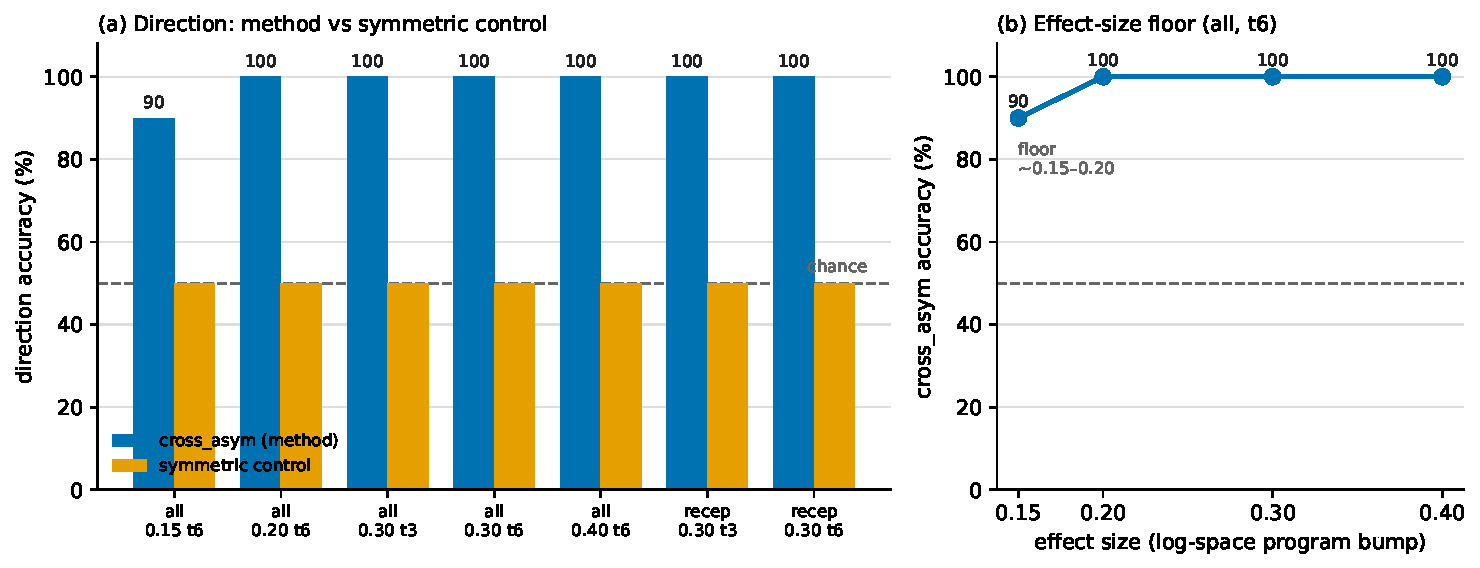
\includegraphics[width=\linewidth]{results_figure.pdf}
\caption{\textbf{(a)} Direction accuracy per configuration: \texttt{cross\_asym} (blue) vs
the confound-corrected symmetric control (orange), with the chance line. \textbf{(b)} The
effect-size detectability floor (mode \texttt{all}, $t\!=\!6$): the weak per-label program
is recovered at $\ge0.20$ and degrades only at $0.15$.}
\label{fig:results}
\end{figure}

\begin{table}[h]
\centering
\caption{Per-configuration results ($1{,}050{,}000$ cells each). \texttt{cross\_asym} and
the symmetric control are the confound-corrected direction accuracies; coupling is measured
by \texttt{signature\_coupling} (donor-level). ``Isolated FP'' counts spuriously-coupled
pairs among the 70 pairs involving a negative-control label.}
\label{tab:main}
\begin{tabular}{@{}llccccccc@{}}
\toprule
mode & eff. & $t$ & \texttt{cross\_asym} & control & coupling recall & coupling FP & isolated FP \\
\midrule
all      & 0.15 & 6 & 90\%  & $\sim$50\% & 100\% & 9\%  & 13/70 \\
all      & 0.20 & 6 & 100\% & $\sim$50\% & 100\% & 8\%  & 13/70 \\
all      & 0.30 & 3 & 100\% & $\sim$50\% & 93\%  & 11\% & 17/70 \\
all      & 0.30 & 6 & 100\% & $\sim$50\% & 100\% & 9\%  & 14/70 \\
all      & 0.40 & 6 & 100\% & $\sim$50\% & 100\% & 10\% & 17/70 \\
receptor & 0.30 & 3 & 100\% & $\sim$50\% & 93\%  & 9\%  & 15/70 \\
receptor & 0.30 & 6 & 100\% & $\sim$50\% & 100\% & 10\% & 16/70 \\
\bottomrule
\end{tabular}
\end{table}

\paragraph{Direction.} \texttt{cross\_asym} recovers the planted direction at 100\% for all
effect sizes $\ge0.20$ and both responder modes, and at 90\% at the weakest effect size; the
symmetric control sits at chance ($\sim$50\%, $\pm16\%$ over random relabelings). This is the
same qualitative result the method shows on real data (88/86/83\% direction vs.\ a
chance-level control), reproduced here on controlled ground truth at $10^6$-cell scale.

\paragraph{Effect-size floor.} The perturbation is deliberately weaker than the cell-type
signature; its detectability floor is $\sim$0.15--0.20 in log space (vs.\ the $\approx$0.9
marker gap), quantifying ``weak but noticeable.''

\paragraph{Depth.} Direction accuracy holds across cascade depth (Table~\ref{tab:depth}):
even the deep chain's weak tail is recovered.

\begin{table}[h]
\centering
\caption{Direction accuracy by cascade depth (source's hops from a root), pooled over
configurations.}
\label{tab:depth}
\begin{tabular}{@{}ccc@{}}
\toprule
source depth & accuracy & edge-observations \\
\midrule
0 & 98\%  & 49 \\
1 & 100\% & 14 \\
2 & 100\% & 7 \\
\bottomrule
\end{tabular}
\end{table}

\paragraph{Coupling and its honest limit.} Signature coupling recovers the truly-coupled
pairs at $\sim$100\% recall at $t\!=\!6$ (93\% at $t\!=\!3$, consistent with deeper edges
emerging later), with an overall false-positive rate of 8--11\%. However, the isolated
negatives are still spuriously flagged as coupled in $\sim$19--24\% of their pairs
(13--17 of 70) even with degree correction --- the known coupling over-call, now quantified
on ground truth.

\section{Conclusion}
\texttt{cascade\_forge} produces controllable single-cell ground truth at million-cell
scale, on which \texttt{cascadir}'s direction call is correct (100\%; 90\% at the weakest
detectable perturbation) while its symmetric control is at chance. The experiment validates
the direction method against a known answer, quantifies its detectability floor, and gives
an honest readout of the coupling over-call on negatives. The one caveat --- and its
resolution --- is a lesson about benchmark hygiene rather than the method: a symmetric
control at 100\% is a design smell, and decoupling label names from cascade order restores
it to chance while leaving the antisymmetric method's 100\% untouched.

\end{document}
